\documentclass[11pt]{article}
\usepackage{amssymb}
\usepackage{fullpage}
\usepackage{comment}
\includecomment{solution}
\excludecomment{question}
\setlength{\parskip}{1ex}
\setlength{\parindent}{0in}
\usepackage{graphicx}
\begin{document}

{\bf \large Quiz 11}
Sebastien Psarianos

\medskip

\begin{question}
Use the subset construction to convert the following NFA with $\lambda$-transitions into a DFA.
Do not include any states that are not reachable from the initial state.

\begin{center}
% \includegraphics{q11-fig.pdf}
\end{center}
\end{question}

\begin{solution}
{\bf Solution}:

\begin{center}
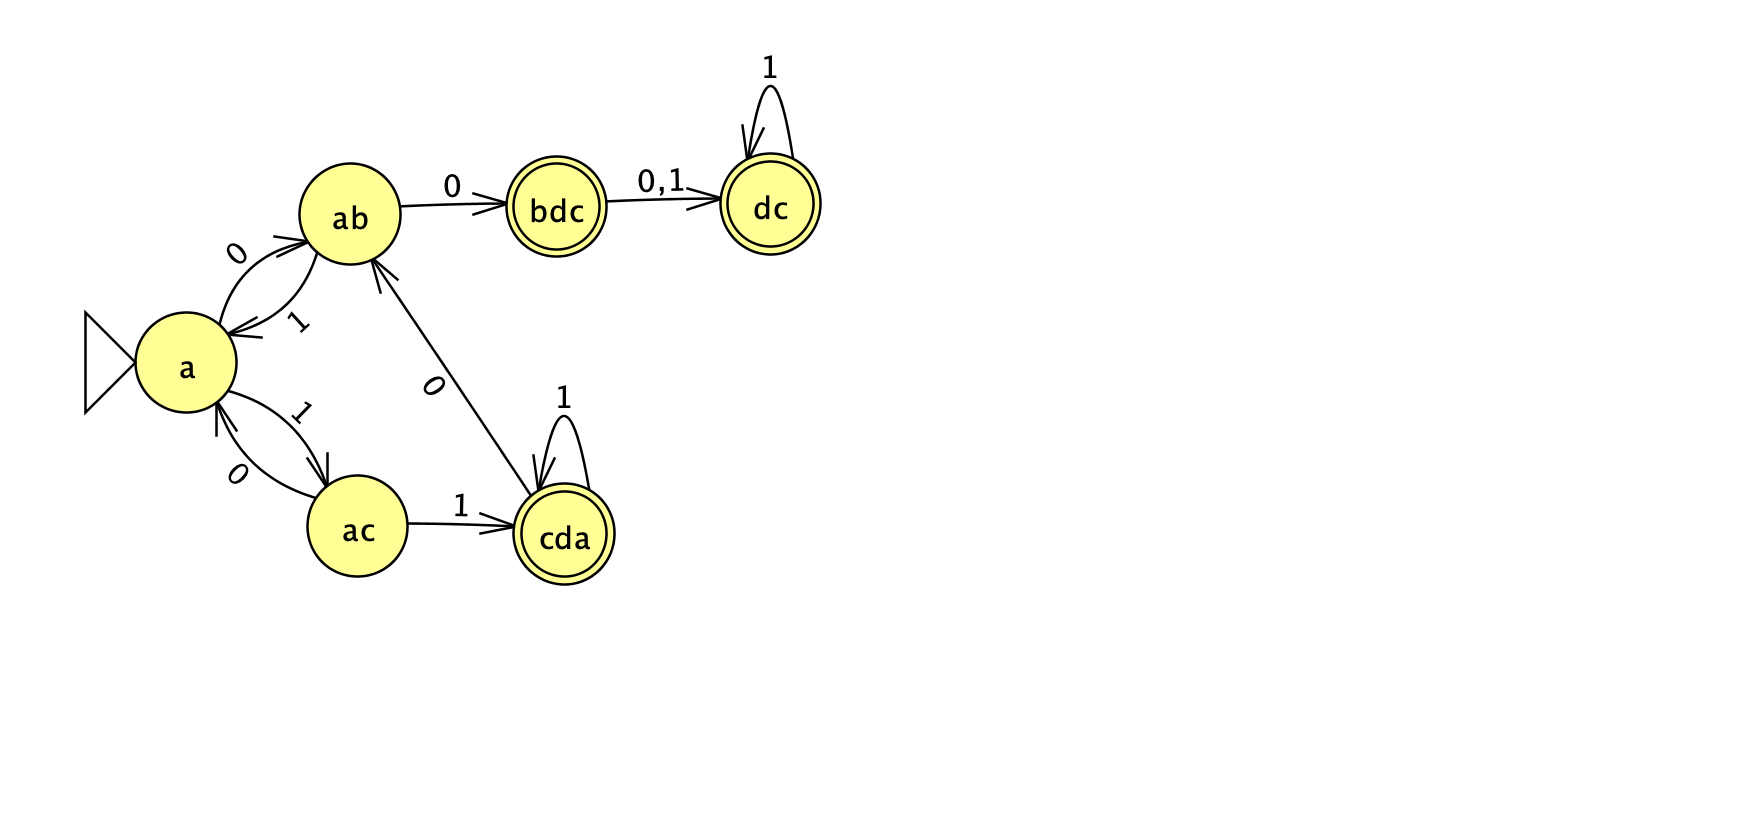
\includegraphics[width=300mm,scale=0.5]{quiz11.png}
\end{center}
\end{solution}
\end{document}
